\documentclass[border=4pt]{standalone}
\usepackage{amsmath,amssymb,amsfonts}
\usepackage{xcolor,colortbl,array,booktabs,multirow}
\usepackage{tikz}
\usetikzlibrary{arrows, automata, backgrounds, calendar, chains, decorations,
    matrix, mindmap, patterns, petri, positioning, shadows, shapes.geometric,
    trees, shapes, decorations.pathreplacing, calc, tikzmark, arrows.meta}
\newcommand{\st}{\text{ s.t. }}
\newcommand{\x}{\mathbf{x}}
\renewcommand{\b}{\mathbf{b}}
\newcommand{\A}{\mathbf{A}}
\newcommand{\R}{\mathbb{R}}
\newcommand{\RR}{\mathbb{R}}
\newcommand{\Z}{\mathbb{Z}}
\newcommand{\ZZ}{\mathbb{Z}}
\begin{document}
\begin{tikzpicture}[
    every node/.style={font=\footnotesize},
    person/.style={circle, draw=blue!50, fill=blue!20, thick, minimum size=1.2cm},
    task/.style={rectangle, draw=red!50, fill=red!20, thick, minimum width=1.2cm, minimum height=1cm}
]

% Nodes for people (drawn stick figures)
\node[person] (P1) at (0, 2) {
    \begin{tikzpicture}
        \draw[thick] (0,0.2) circle (0.15); % Head
        \draw[thick] (0,0.05) -- (0,-0.2);  % Body
        \draw[thick] (-0.1,-0.3) -- (0,-0.2) -- (0.1,-0.3); % Legs
        \draw[thick] (-0.1,0) -- (0.1,0);   % Arms
    \end{tikzpicture}
    \\ $P_1$
};

\node[person] (P2) at (0, 0) {
    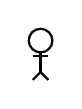
\begin{tikzpicture}
        \draw[thick] (0,0.2) circle (0.15);
        \draw[thick] (0,0.05) -- (0,-0.2);
        \draw[thick] (-0.1,-0.3) -- (0,-0.2) -- (0.1,-0.3);
        \draw[thick] (-0.1,0) -- (0.1,0);
    \end{tikzpicture}
    \\ $P_2$
};

\node[person] (P3) at (0, -2) {
    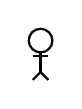
\begin{tikzpicture}
        \draw[thick] (0,0.2) circle (0.15);
        \draw[thick] (0,0.05) -- (0,-0.2);
        \draw[thick] (-0.1,-0.3) -- (0,-0.2) -- (0.1,-0.3);
        \draw[thick] (-0.1,0) -- (0.1,0);
    \end{tikzpicture}
    \\ $P_3$
};

% Nodes for tasks (drawn clipboard-like symbols)
\node[task] (T1) at (4, 2) {
    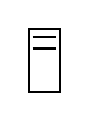
\begin{tikzpicture}
        \draw[thick] (-0.2,0.4) rectangle (0.2,-0.4); % Task shape
        \draw[thick] (-0.15,0.3) -- (0.15,0.3); % Line inside
        \draw[thick] (-0.15,0.15) -- (0.15,0.15);
    \end{tikzpicture}
    \\ $T_1$
};

\node[task] (T2) at (4, 0) {
    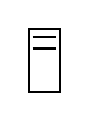
\begin{tikzpicture}
        \draw[thick] (-0.2,0.4) rectangle (0.2,-0.4);
        \draw[thick] (-0.15,0.3) -- (0.15,0.3);
        \draw[thick] (-0.15,0.15) -- (0.15,0.15);
    \end{tikzpicture}
    \\ $T_2$
};

\node[task] (T3) at (4, -2) {
    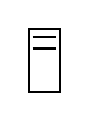
\begin{tikzpicture}
        \draw[thick] (-0.2,0.4) rectangle (0.2,-0.4);
        \draw[thick] (-0.15,0.3) -- (0.15,0.3);
        \draw[thick] (-0.15,0.15) -- (0.15,0.15);
    \end{tikzpicture}
    \\ $T_3$
};

% Edges (Complete bipartite graph)
\foreach \i in {1,2,3} {
    \foreach \j in {1,2,3} {
        \draw[thick] (P\i) -- (T\j);
    }
}

\end{tikzpicture}
\end{document}
